% ------------------------------------------------------------------- %
%  Studi Literature / Kajian Pustaka / Literature Review
%  AUTHOR: @NoHaitch IF'22
%  DATE: 2026-05-16
% ------------------------------------------------------------------- %

% -------------------- II --------------------
\chapter{Studi Literatur}
\label{2-Studi-Literatur}
% -------------------- II --------------------

\todo{
    Bab Studi Literatur digunakan untuk mendeskripsikan kajian literatur yang terkait dengan persoalan tugas akhir. Tujuan studi literatur adalah:

    \begin{enumerate}
        \item menunjukkan kepada pembaca adanya gap seperti pada rumusan masalah yang memang belum terselesaikan,
        \item memberikan pemahaman yang secukupnya kepada pembaca tentang teori atau pekerjaan terkait yang terkait langsung dengan penyelesaian persoalan, serta
        \item menyampaikan informasi apa saja yang sudah ditulis/dilaporkan oleh pihak lain (peneliti/Tugas Akhir/Tesis) tentang hasil penelitian/pekerjaan mereka yang sama/mirip/erat kaitannya dengan persoalan tugas akhir.
    \end{enumerate}

    % -------------------- II.1 --------------------
    \section{Contoh Subbab}
    % -------------------- II.1 --------------------

    Contoh subbab.

    % -------------------- II.1.1 --------------------
    \subsection{Contoh Referensi Sitasi}
    % -------------------- II.1.1 --------------------

    Referensi diletakan pada format biblitext dalam file `references.bib`

    Referensi disitasi menggunakan format APA dengan `cite\{\}` atau `parencite\{\}'

    Contoh: \\
    Publikasi ilmiah sudah berkembang dari abad ke-17, dengan terbitnya \textit{Philosophical Transactions} oleh Royal Society \parencite{fyfe2022}.

    % -------------------- II.1.1.1 --------------------
    \subsubsection{Contoh Gambar}
    % -------------------- II.1.1.1 --------------------

    Contoh gambar adalah sebagaimana terlihat pada Gambar~\ref{fig:contoh-inline}, 

    % -------------------- II.1.1.1.1 --------------------
    \paragraph{Gambar.}
    % -------------------- II.1.1.1.1 --------------------

    \begin{center}
        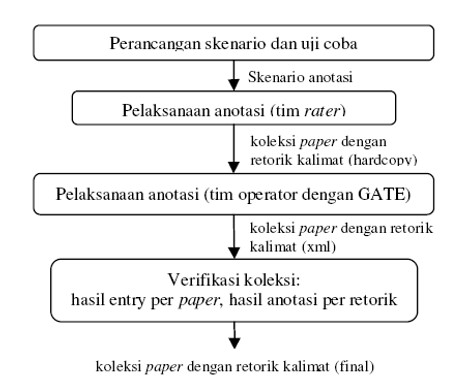
\includegraphics[width=0.8\textwidth]{images/example.jpg}
        \captionof{figure}{Tahapan konstruksi koleksi retorik kalimat}
        \label{fig:contoh-inline}
    \end{center}


    % -------------------- II.1.1.1.2 --------------------
    \paragraph{Contoh Tabel}
    % -------------------- II.1.1.1.2 --------------------

    Data dapat dilihat pada Tabel~\ref{tab:contoh-merge} berikut.
    
    \begin{xltabular}{\textwidth}{|c|X|c|}
        \caption{Contoh Tabel}
        \label{tab:contoh-merge} \\
        \hline
        \rowcolor[HTML]{EFEFEF}
        \textbf{No.} & \multicolumn{1}{c|}{\textbf{Kegiatan}} & \multicolumn{1}{c|}{\textbf{Waktu Pelaksanaan}} \\
        \hline
        \endfirsthead
        \multicolumn{3}{c}{{\tablename\ \thetable{}: Contoh Tabel (lanjutan)}} \\
        \hline
        \rowcolor[HTML]{EFEFEF}
        \textbf{No.} & \multicolumn{1}{c|}{\textbf{Kegiatan}} & \multicolumn{1}{c|}{\textbf{Waktu Pelaksanaan}} \\
        \hline
        \endhead
        \hline
        \multicolumn{3}{r}{\textit{Bersambung ke halaman berikutnya}} \\
        \endfoot
        \hline
        \endlastfoot  
        
        % Multi-row example
        \multirow{2}{*}{1} & Studi Literatur & Januari 2025 \\ \cline{2-3}
            & Analisis Kebutuhan & Februari 2025 \\ \hline

        % Normal row
        2 & Perancangan Sistem & Maret 2025 \\ \hline

        % Multi-column example
        3 & \multicolumn{2}{c|}{Implementasi dan Pengujian (April–Mei 2025)} \\ \hline

        % Normal row + Multi page table
        4 & Dokumentasi & Juni 2025 \\ \hline
        4 & Dokumentasi & Juni 2025 \\ \hline
        4 & Dokumentasi & Juni 2025 \\ \hline
        4 & Dokumentasi & Juni 2025 \\ \hline
        4 & Dokumentasi & Juni 2025 \\ \hline
        4 & Dokumentasi & Juni 2025 \\ \hline
        4 & Dokumentasi & Juni 2025 \\ \hline
        4 & Dokumentasi & Juni 2025 \\ \hline
        4 & Dokumentasi & Juni 2025 \\ \hline
        4 & Dokumentasi & Juni 2025 \\ \hline
        4 & Dokumentasi & Juni 2025 \\ \hline
        4 & Dokumentasi & Juni 2025 \\ 
    \end{xltabular}

} 

% end Todo
